\documentclass[a4paper]{article}
\usepackage[a4paper]{geometry}
\usepackage{pdfpages}
\begin{document}
\section*{Mixed School Problem Solving Questions}

1. Express the four digit number as $ABCD$, then $$1000A + 100B + 10C + D + 1000D + 100C + 10B + A = 11(91A + 10B + 10C + 91D).$$ 
2. Solve $6x-0.5x=90$ \\
3. Counting gives 27. \\
4. a) $x=2$ \\
5. Let $\frac{p}{q}$ be the smallest element, then $\frac{p}{q+1} < \frac{p}{q}$ and we have a contradiction. \\
6. a) no b) yes\\
7. Let the weights be $a \le b \le c \le d$. Then $a + b = 89$ since it
is the smallest sum, $b + d = 120$ since it is the second largest sum. Hence
$d - a = b + d - (a + b) = 120 - 89 = 31kg$.
(The possible weights are 41, 48, 64, 72 or 40.5, 48.5, 64.5, 71.5.)
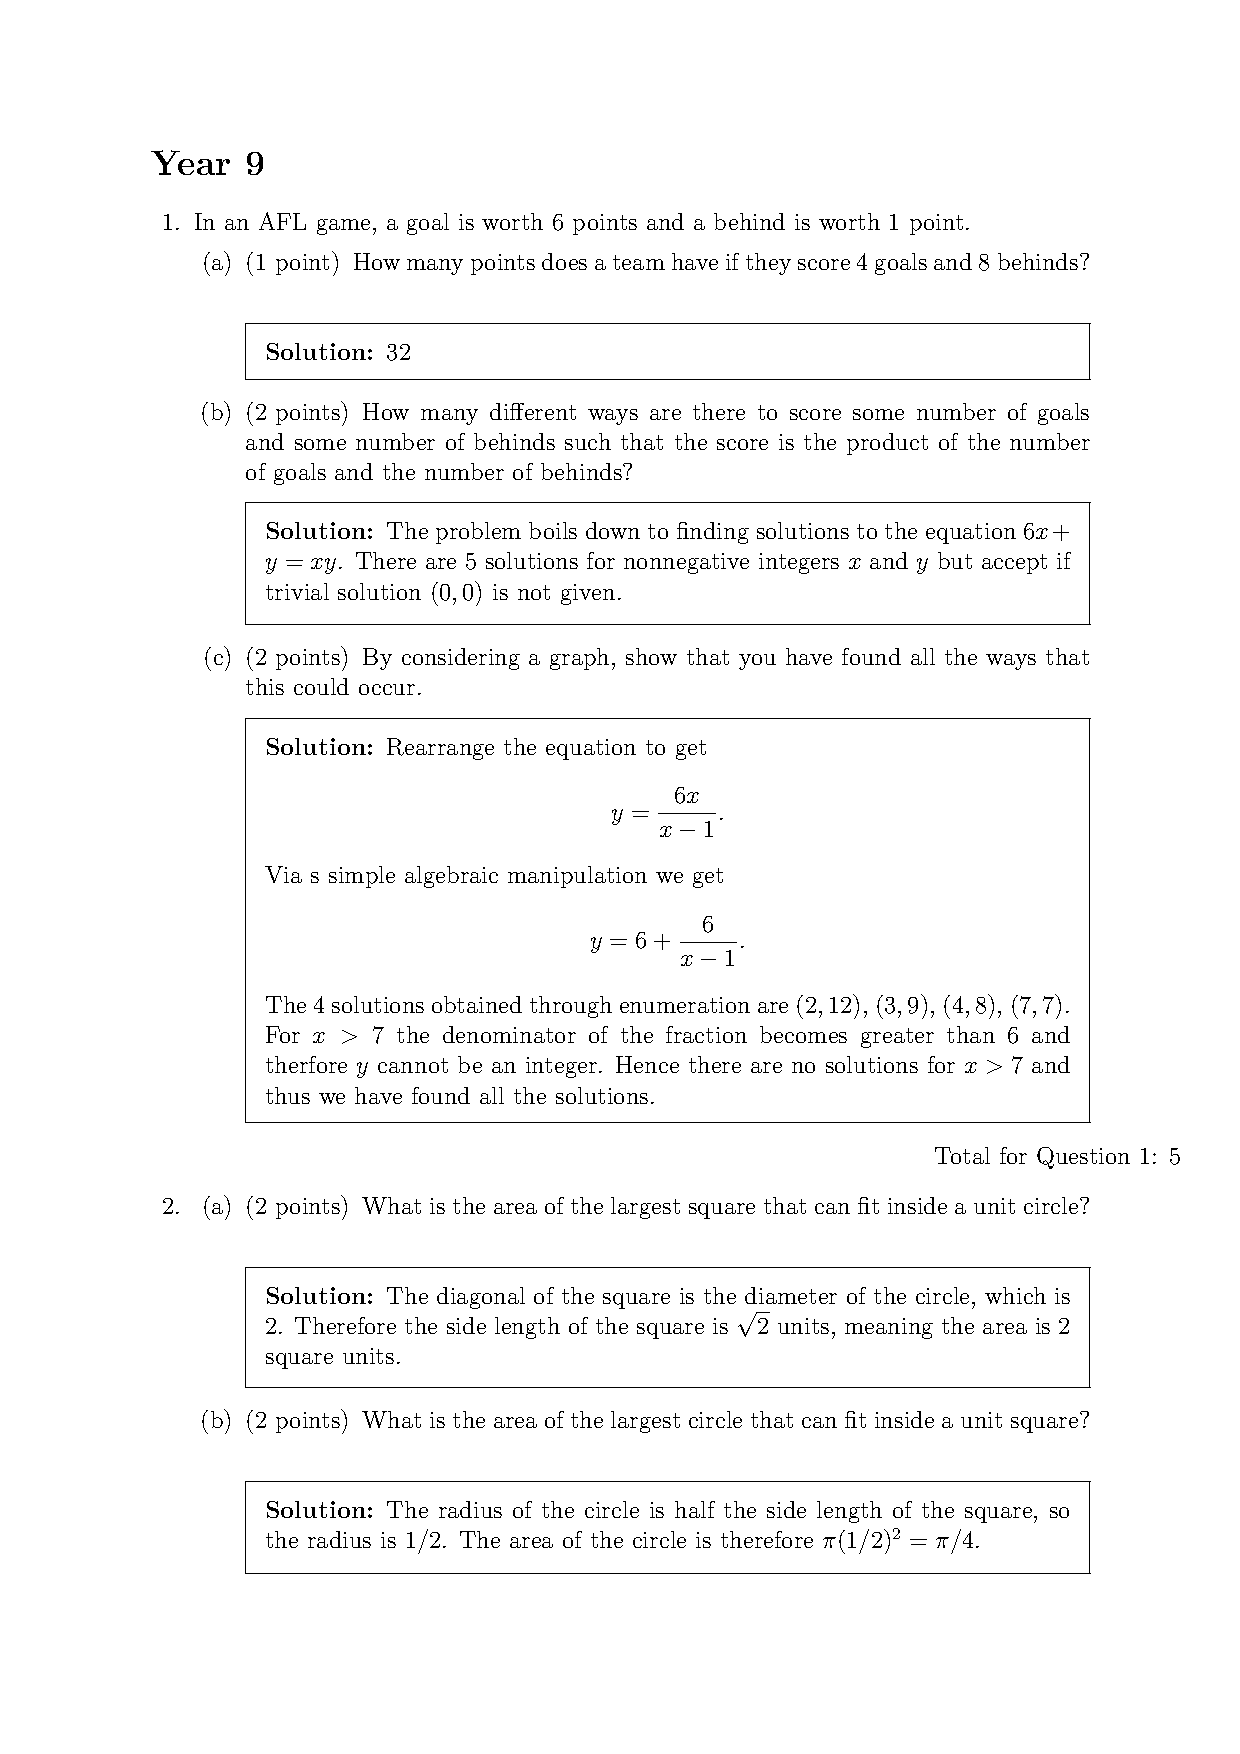
\includepdf[pages=-]{SEHS_Maths_Games_Day_2023_Problem_Solving_Year9_Solutions}
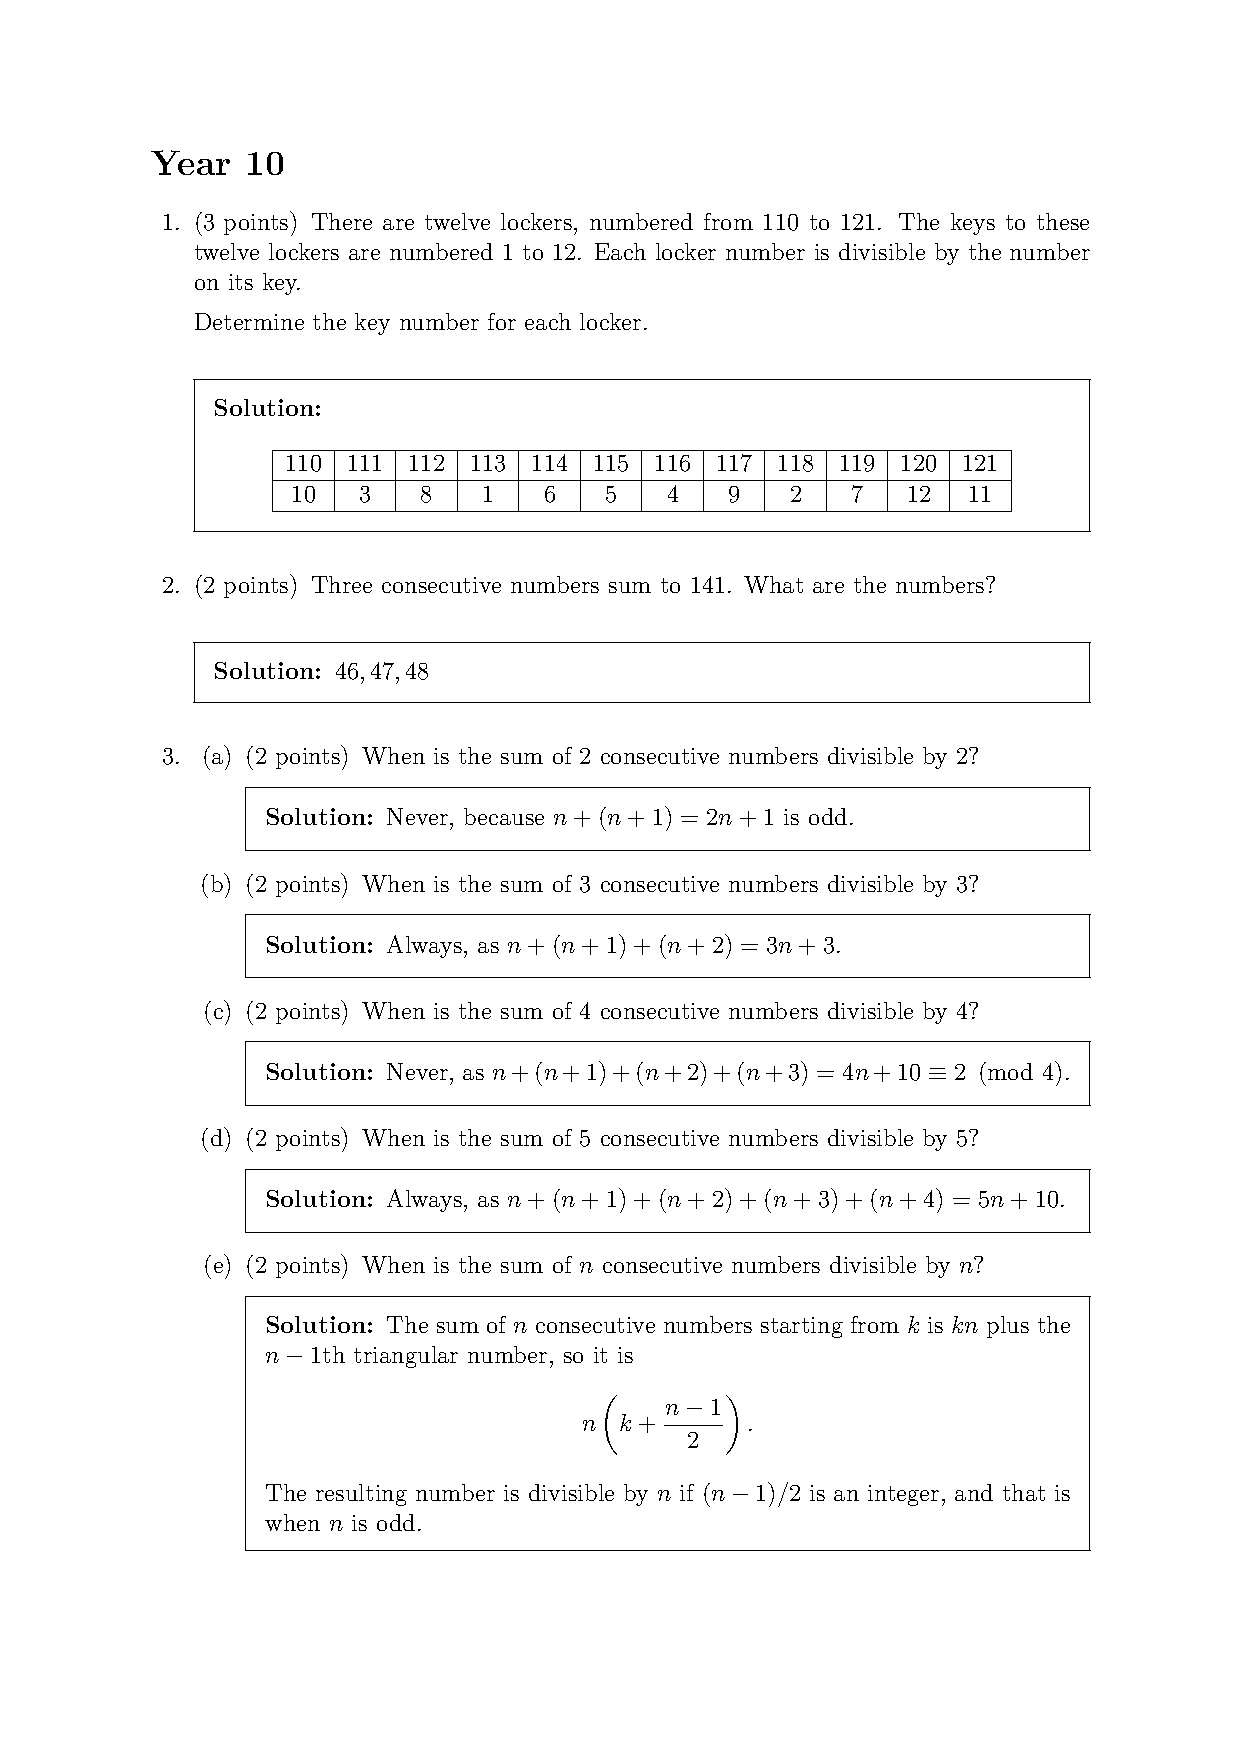
\includepdf[pages=-]{SEHS_Maths_Games_Day_2023_Problem_Solving_Year10_Solutions}
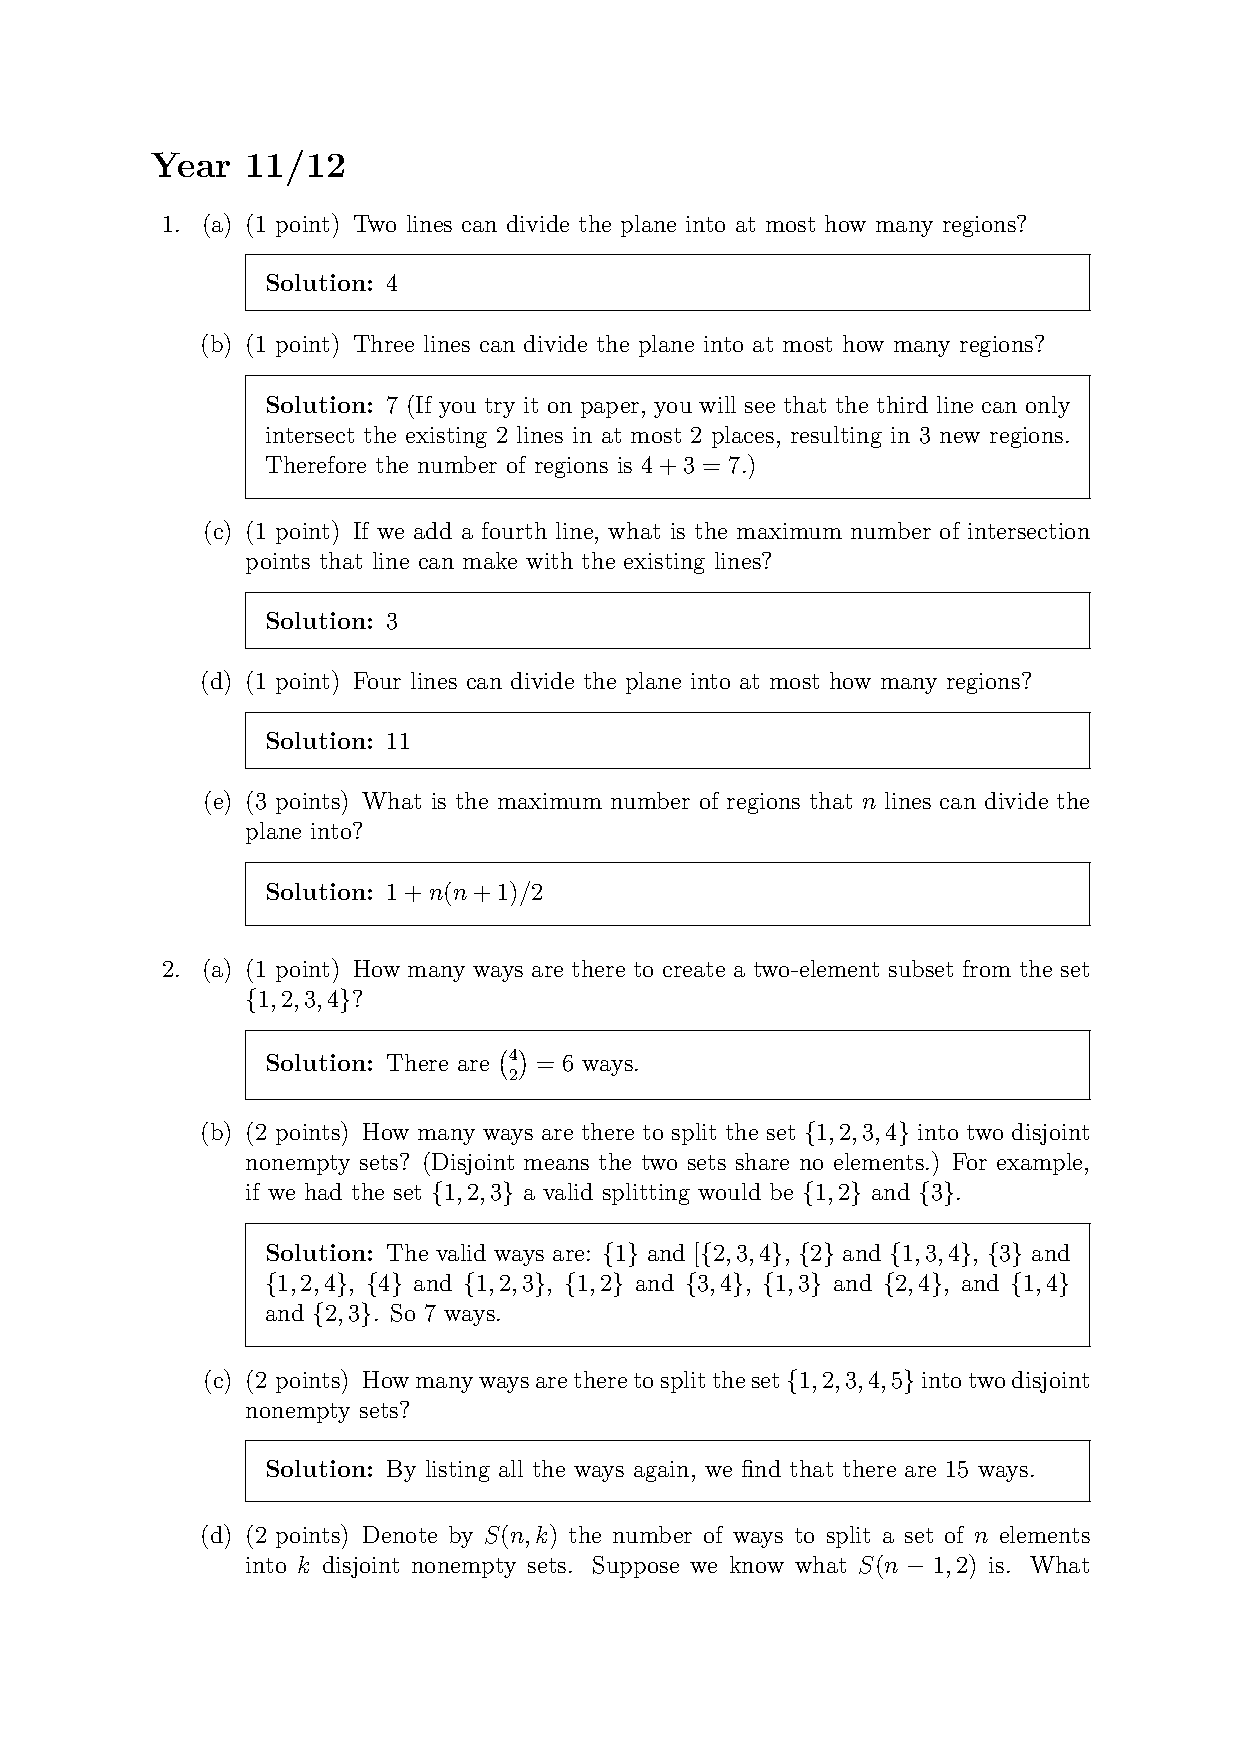
\includepdf[pages=-]{SEHS_Maths_Games_Day_2023_Problem_Solving_Year11-12_Solutions}
\end{document}